\section{Results}
\label{sec:results}

In this section, we present the results of our evaluation of production validation outcomes across the benchmark. We begin by examining overall acceptance behavior and then analyze reliability, convergence dynamics, and validation characteristics across models.


\subsection{Primary Outcome: Production Validation Acceptance}
Across all 604 prompt-level trials (151 prompts for each of four models), single-shot production validation succeeded for 309/604 cases (51.16\%). Under validator-in-the-loop refinement, pipeline production validation succeeded for 604/604 cases (100.00\%).

\begin{figure}[H]
\centering
% Figure 2 options (pick one):
% \input{results/figures/01_overall_option_b_dumbbell}
% \input{results/figures/01_overall_option_c_stacked_gain}
\input{results/figures/01_overall_option_a_horizontal}
\caption{Overall single-shot vs final pipeline production-validation acceptance across all 604 prompt-level cases.}
\label{fig:overall_baseline_vs_pipeline}
\end{figure}

\subsection{Per-Model Reliability}
All models reached 151/151 eventual production validation under the validator-gated loop, but single-shot pass rates differed substantially. Figure~\ref{fig:by_model_baseline_vs_pipeline} provides the per-model comparison with exact acceptance values annotated on the bars.

\begin{figure}[H]
\centering
\input{results/figures/02_baseline_vs_pipeline_compile_rate_by_model}
\caption{Per-model single-shot vs final pipeline production-validation acceptance.}
\label{fig:by_model_baseline_vs_pipeline}
\end{figure}

Anthropic Sonnet 4.6 had the highest single-shot pass rate (82.78\%), while OpenAI Codex 5.2 (41.72\%), DeepSeek Reasoner (41.06\%), and Mistral Large (39.07\%) showed worse single-shot behavior and larger single-shot-to-pipeline gaps.

\subsection{Convergence Behavior}
Convergence is indexed by repair cycles: $k=0$ denotes the initial single-shot generation (no validator feedback), and $k\geq 1$ denotes validator-guided repair cycles; acceptance corresponds to zero-error output under the production validator.

Figure~\ref{fig:cumulative_convergence} first presents the pooled convergence trajectory across all prompt-level cases.

\begin{figure}[H]
\centering
\input{results/figures/03_cumulative_acceptance_by_iteration}
\caption{Cumulative production-validation acceptance versus repair cycles ($k$). $k=0$ denotes initial single-shot generation; $k\geq 1$ denotes validator-guided repair cycles. Acceptance corresponds to zero-error output under the production validator.}
\label{fig:cumulative_convergence}
\end{figure}

The pooled curve shows a large first-step jump from $k=0$ to $k=1$, followed by rapid compression by $k=2$ and then a short tail. Table~\ref{tab:convergence_behavior} provides the exact counts and percentages underlying Figure~\ref{fig:cumulative_convergence}: acceptance increases from 51.16\% at $k=0$ to 84.44\% at $k=1$, reaches 94.37\% by $k=2$, and reaches 99.67\% by $k=4$. Only two cases remain in the grouped $k=5$--$8$ tail (0.33\%), where cumulative acceptance reaches 100.00\%. Consistent with this front-loaded pattern, iterations-to-acceptance are summarized by mean 1.727, median 1, IQR 1--2, and maximum 8.

\input{results/tables/table_convergence_behavior}

\noindent\textbf{Rate Characterization.} To quantify the observed convergence shape, we report an empirical contraction analysis of residual failure mass. Under contraction-style iteration analysis, let residual failure mass be $R_k = 1 - A_k$. The observed residual sequence is $R_0=0.4884$, $R_1=0.1556$, $R_2=0.0563$, $R_3=0.0182$, and $R_4=0.0033$. Using early cycles, the empirical contraction ratios are $\rho_0 \approx 0.1556/0.4884 \approx 0.32$, $\rho_1 \approx 0.0563/0.1556 \approx 0.36$, and $\rho_2 \approx 0.0182/0.0563 \approx 0.32$. These values cluster around an average early-cycle contraction factor of approximately 0.33 (computed as the arithmetic mean of $\rho_0$--$\rho_2$). Tail transitions are excluded from contraction-rate estimation because ratios become unstable when residual mass is near the finite-sample resolution. These early-cycle ratios cluster in a narrow band, suggesting an approximately multiplicative (``contraction-like'') reduction pattern in the initial repair regime. In practical terms, early cycles remove roughly two-thirds of the remaining failures per cycle (in the observed early regime).

Complementing the contraction estimate, time-to-threshold metrics quantify convergence speed. The observed thresholds are $T_{90}=2$, $T_{95}=3$, and $T_{99}=4$. These values characterize how rapidly validator-guided refinement approaches the acceptance set in repair-cycle space.

To assess whether this pooled behavior is shared across backends, Figure~\ref{fig:cumulative_convergence_by_model} overlays per-model cumulative acceptance trajectories.

\begin{figure}[H]
\centering
\input{results/figures/04_cumulative_acceptance_by_model_overlay}
\caption{Per-model cumulative production-validation acceptance versus repair cycles ($k$).}
\label{fig:cumulative_convergence_by_model}
\end{figure}

Figure~\ref{fig:cumulative_convergence_by_model} shows that single-shot starting points differ across models, but the trajectories compress rapidly once validator-guided repair begins. Despite different initial acceptance levels, all curves move quickly toward full acceptance within a small number of repair cycles. This pattern supports the model-agnostic control-signal interpretation: deterministic validator diagnostics drive the dominant convergence dynamics across backends.

\subsection{Statistical Reliability}

We now quantify the reliability of validator-guided convergence across the full campaign. In total, we evaluated $n=604$ prompt--model cases. In single-shot generation, 309 of 604 cases (51.16\%) passed production validation. Under validator-guided refinement, all 604 cases ultimately reached zero-error production acceptance, with no observed failures.

To interpret this result statistically, we model convergence as a Bernoulli process and compute an exact 95\% Clopper--Pearson lower confidence bound on the convergence probability $p$~\cite{clopper1934confidenceLimits}. For the all-success case ($x=604$ successes in $n=604$ trials), the lower bound is
\[
p_L = (\alpha/2)^{1/n},
\]
with $\alpha=0.05$. Substituting $n=604$ gives
\[
p_L = (0.025)^{1/604} \approx 0.9939.
\]
With 95\% confidence, the true convergence probability under this benchmark configuration is therefore at least 99.39\%.

Equivalently, we can compute a one-sided 95\% upper bound on the failure probability $q=1-p$ by solving $(1-q)^n=0.05$. For $n=604$, this yields
\[
q_U = 1 - 0.05^{1/604} \approx 0.00495,
\]
or approximately 0.495\%. A large-$n$ approximation gives $q_U \approx -\ln(0.05)/604 \approx 0.00496$, which is consistent with the exact calculation. 

In practical terms, this means that even though we observed zero failures in 604 cases, statistical uncertainty remains finite. Based on the binomial confidence analysis, we can state with 95\% confidence that the true failure rate under this benchmark configuration is below approximately 0.5\%, and equivalently that the true convergence probability exceeds 99\%. While this does not imply perfect reliability, it indicates that production-validator convergence is highly probable for SysMBench-style prompts under the evaluated setup.

We emphasize that these bounds apply to SysMBench-style prompt distributions under the evaluated controller, validator, and backend configuration. They do not imply universal convergence over arbitrary natural-language inputs. At the same time, the absence of observed failures is consistent with the structure of the loop. Accepted cases terminate immediately, and rejected cases receive deterministic diagnostics that guide subsequent revisions. Within this benchmark distribution, validator-gated refinement exhibits stable and highly reliable convergence behavior.

\subsection{Grammar Validity vs. Production Validity and Error Burden}

In practice, a SysMLv2 artifact must pass production validation in a modeling environment before it can be used downstream. Grammar parsability alone is not sufficient. To quantify the gap between these two notions of validity, we compared ANTLR parsing outcomes against production validation outcomes for the initial candidate ($k=0$) across all 604 prompt--model cases.

Of the 604 initial candidates, 369 (61.09\%) passed grammar-level parsing, whereas only 309 (51.16\%) passed production validation. In 60 cases, the generated model passed ANTLR parsing but failed production validation. These 60 cases represent 16.26\% of grammar-valid artifacts (60/369) and 9.93\% of all initial outputs (60/604). In other words, grammar-level parsing overestimates operational usability by approximately 16\% among parseable artifacts. We did not observe any case in which a model passed production validation while failing grammar parsing (0/604), indicating that grammar validity is necessary but not sufficient for production acceptance under the evaluated configuration.

\begin{figure}[H]
\centering
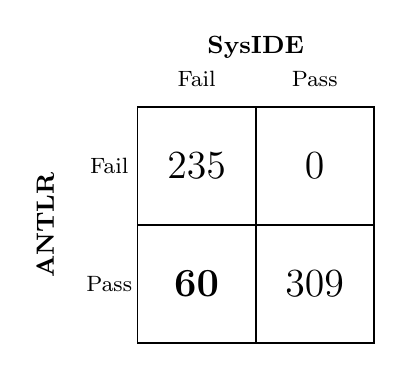
\begin{tikzpicture}[x=1.5cm,y=1.5cm]
\draw[line width=0.65pt] (0,0) rectangle (2,2);
\draw[line width=0.65pt] (1,0) -- (1,2);
\draw[line width=0.65pt] (0,1) -- (2,1);

% Axis labels and definitions
\node[font=\small\bfseries] at (1.0,2.50) {SysIDE};
\node[font=\footnotesize] at (0.5,2.24) {Fail};
\node[font=\footnotesize] at (1.5,2.24) {Pass};

\node[font=\small\bfseries, rotate=90] at (-0.78,1.0) {ANTLR};
\node[font=\footnotesize, align=right] at (-0.24,1.5) {Fail};
\node[font=\footnotesize, align=right] at (-0.24,0.5) {Pass};

% Cell values (top row: ANTLR fail, bottom row: ANTLR pass)
\node[font=\Large] at (0.5,1.5) {235};
\node[font=\Large] at (1.5,1.5) {0};
\node[font=\Large] at (0.5,0.5) {\textbf{60}};
\node[font=\Large] at (1.5,0.5) {309};

\end{tikzpicture}
\caption{Initial-candidate grammar (ANTLR) vs production validation (SysIDE), $n=604$. The operational-gap cell (ANTLR pass, SysIDE fail) contains 60 cases.}
\label{fig:antlr_vs_production_flow}
\end{figure}



%We also examined the validator error burden for initial candidates. Across all 604 cases, the production validator reported a total of 2,209 errors, corresponding to a mean of 3.66 errors per generated model. Restricting to the 295 cases that failed production validation, the mean error burden increases to 7.49 errors per failing model. These values indicate that failures typically involve multiple structural inconsistencies rather than isolated formatting mistakes.

%The distribution of error types further clarifies this pattern. Parsing errors account for 1,144 of the 2,209 total errors (51.79\%), while reference errors account for 824 (37.30\%). Together, these two categories comprise 89.09\% of all initial-candidate errors. This concentration suggests that many initial outputs contain compound structural defects, including unresolved references and incomplete declarations. Grammar-level parsing alone would admit a subset of these artifacts into downstream workflows, despite their inability to pass production validation. Validator-guided repair therefore addresses not only token-level syntax issues, but broader structural inconsistencies that affect operational usability.


\subsection{Insights from Extended Analyses}
\textbf{First, we observe no meaningful relationship between iterations-to-success and either SysMBench difficulty or the length of the generated SysML output. Repair effort therefore does not appear to scale with model size or benchmark difficulty. One possible explanation is that raw line count does not capture the number of distinct grammatical structures that must be correctly formed; shorter outputs may still contain complex reference or typing relationships that trigger validator failures.
Second, when validator errors persist across repair iterations, the majority occur because the LLM does not modify the validator-highlighted code region at all, effectively ignoring the reported diagnostic. In the remaining cases, the model appears to attempt a repair but produces another invalid construction. This pattern suggests both a pipeline efficiency gap, in which repair iterations are wasted when the highlighted region is not revised, and a model limitation, in which the model attempts a repair but fails to generate a syntactically valid correction.}

\subsection{Open-Source Dataset Release}

We release the full trajectory-level corpus generated in this study rather than only baseline and final artifacts. The dataset spans the complete SysMBench prompt set of 151 prompts evaluated across four model backends, yielding 604 prompt--model cases. For each case, we retain every validator-guided refinement step. In total, the release contains 1,043 stored iteration artifacts. Each artifact includes the generated SysMLv2 text and the corresponding production-validator diagnostics. As a result, the dataset preserves the full correction trajectory for each case, not just its endpoints.

At the artifact level, we classify iterations as positive if they pass production validation and negative if they fail. Under this definition, the release contains 604 positive artifacts and 439 negative artifacts. For a newly standardized language such as SysMLv2, where publicly available corpora of production-accepted models remain limited, these 604 positive artifacts provide a meaningful resource. The 439 negative artifacts correspond to intermediate repair states within the same 604 trajectories; they do not represent additional independent benchmark instances, but rather the correction path taken for each prompt--model pair.

%The negative artifacts are rarely trivial failures. Across all iteration artifacts, the validator reports 3,232 total error instances. When restricted to failing artifacts only, the mean error burden is 7.36 errors per artifact, with a median of 4.00 and a maximum of 267 errors in a single case. The maximum observed trajectory depth is eight iterations, and the mean number of iterations per case is 1.73. These statistics indicate that failing states typically involve multiple structural inconsistencies rather than isolated formatting issues, and that repair often requires resolving several interacting errors.

Releasing full stepwise traces enables analyses that are not possible with endpoint-only datasets. Researchers can study repair dynamics under deterministic validator feedback, model convergence behavior across trajectories, and explore learning strategies that operate on intermediate states rather than final outputs alone. Because we retain runtime and token-level metadata at both iteration and trajectory levels, the dataset also supports systematic cost--reliability tradeoff analyses under a consistent production-validation criterion.
